\documentclass[11pt,a4paper]{article}

\usepackage[T1]{fontenc}
\usepackage{lmodern}
\usepackage[margin=1in]{geometry}
\usepackage{amsmath,amssymb,amsthm,mathtools}
\usepackage{graphicx}
\usepackage{booktabs}
\usepackage{xcolor}
\usepackage{listings}
\usepackage{tcolorbox}
\tcbuselibrary{listings,skins,breakable}
\usepackage{microtype}
\usepackage{hyperref}
\hypersetup{colorlinks=true,linkcolor=blue,citecolor=blue,urlcolor=blue}
\usepackage{pgfplots}
\pgfplotsset{compat=1.18}
\usepackage{tikz}

% Theorem environments
\newtheorem{lemma}{Lemma}
\newtheorem{theorem}{Theorem}
\newtheorem{corollary}{Corollary}
\theoremstyle{remark}
\newtheorem{remark}{Remark}

% Listings setup
\definecolor{leanbg}{rgb}{0.97,0.97,0.99}
\definecolor{leankw}{rgb}{0.10,0.20,0.60}
\definecolor{leancm}{rgb}{0.30,0.50,0.30}
\definecolor{leanst}{rgb}{0.60,0.20,0.20}

\lstdefinelanguage{lean}{
  morekeywords={theorem,lemma,def,noncomputable,structure,by,unfold,rfl,sorry,
                Nat,Type,DecidableEq,Finset,Clause,Sym2,List,Prop,where,
                pending},
  sensitive=true,
  morecomment=[l]{--},
  morecomment=[s]{/-}{-/},
  morestring=[b]"
}

\lstset{
  basicstyle=\ttfamily\footnotesize,
  keywordstyle=\color{leankw}\bfseries,
  commentstyle=\color{leancm}\itshape,
  stringstyle=\color{leanst},
  backgroundcolor=\color{leanbg},
  breaklines=true,
  breakatwhitespace=true,
  columns=fullflexible,
  showstringspaces=false,
  frame=single,
  framesep=4pt,
  xleftmargin=4pt,
  xrightmargin=4pt
}

\title{Cumulative Active-Clause Entropy as a Computable Proxy for Resolution
Cumulative Space: An Honest Empirical Localisation on Tseitin and Structured
Families}

\author{Ludovico Kubler\thanks{Independent researcher;
ludwigkubler.ia at gmail dot com}}

\date{June 2026}

\begin{document}

\maketitle

\begin{abstract}
We study a computable, per-trace functional
$\Phi_{\mathrm{count}}(\pi) := \sum_t |M_t|$ --- the sum over a
Davis--Putnam refutation trace of the active-clause-set size at each step ---
and its relationship to the formula-level invariant
$\mathrm{CSpace}_{\mathrm{cum}}(F)$ of Alwen, de Rezende, Nordstr\"om and
Vinyals (ITCS 2017, paper 38; henceforth ADRNV)~\cite{ADRNV2017}. Our
contribution is \textbf{an honest empirical localisation}, \emph{not} a
complexity-theoretic separation. We (i) state Lemma A in its honest two-part
form --- a near-tautological per-trace identity discharged by definitional
unfolding in Lean 4, plus a corrected formula-level
\textbf{schedule-bookkeeping inequality}
$\Phi_{\mathrm{count}}^{\mathrm{DP},h}(F) \le
\mathrm{CSpace}_{\mathrm{cum}}(\pi'_{\mathrm{DP},h})$ via a primitive
expansion of the DP macro-trace --- and \textbf{retract} the v4 reverse
direction $\Phi_{\mathrm{count}} \ge \mathrm{CSpace}_{\mathrm{cum}}$, which
v4 derived from an erroneous one-line min-over-traces argument; (ii) report
a pre-registered measurement campaign with cluster-robust model selection
and paired-by-seed bootstrap. The combined DP-min-occurrence corpus on
rand-3-regular Tseitin over $n \in \{14, 22, 30, 32, 34, 36\}$ gives a
log-log slope $\widehat\alpha_{\Phi} = 4.43$, \textbf{up from the v3 figure
of 3.43 on $n = 10\text{--}30$} and continuing to drift upward across
windows (2.42 $\to$ 2.93 $\to$ 3.43 $\to$ 4.43); the $n=36$ point is
left-censored (3 of 10 instances \texttt{BLEW\_UP} at
$\mathrm{MAX\_DB} = 1.5 \times 10^6$), biasing the slope
\textbf{downward}, with a Tobit correction flagged as future work. Per the
corrected Lemma A, this exponent is reported as a
\textbf{schedule-specific measurement with no formal ordering to
$\mathrm{CSpace}_{\mathrm{cum}}$}, not as an upper witness.
(iii) The DRAT/DP gap is confirmed on paired-by-seed instances:
$\widehat\alpha_{\mathrm{DRAT,default}} -
\widehat\alpha_{\mathrm{DP,min\text{-}occ}} \approx 3.28 \pm 0.4$
on $n \in \{14, 22, 30\}$. (iv) The v3 mechanism narrative for that gap
--- ``inprocessing eliminates clauses, hence lower DRAT $\Phi$'' --- is
\textbf{retracted}. A flag-by-flag decomposition on $n \in \{10, \ldots, 60\}$
with a paired-by-seed cluster bootstrap (B=2000) shows the no-restart
effect \emph{survives} with full-range CI $[+0.213, +0.435]$ but is fragile:
excluding the $n=60$ cell collapses the shift to $+0.07$ $[+0.03, +0.11]$.
No-inprocessing is reported as suggestive ($+0.14$ $[+0.07, +0.18]$ full
range; CI crosses zero without $n=60$). No-eliminate is null. Roughly 10\%
of the DRAT/DP exponent gap is attributable to restart strategy, with the
caveat that the signal is concentrated at $n=60$.
(v) On $Q_5$ Tseitin, DP-min-occurrence deterministically aborts at step
37 with final database $2^{20}$ at $\mathrm{MAX\_DB} = 4 \times 10^6$
across all three seeds; the $Q_5$ slope is therefore
\textbf{not measurable} under this heuristic, and the v3 ``treewidth not
degree'' framing is reframed as a structural negative.
(vi) On random-4-regular Tseitin (DP-infeasible: 5/5 \texttt{BLEW\_UP} at
$n=16$), kissat-DRAT gives slope 7.69 on $n \in \{16, 20, 24, 28\}$; this
closes the v3 symmetric-comparison defect at the cost of a proof-system
confound (DP on $Q_4$ vs DRAT on rand\_4reg), which we acknowledge rather
than wave away. The headline reading of this paper is: \textbf{a
cumulative-entropy proxy $\Phi$ for resolution refutations on Tseitin
formulas, with a measured exponent $\widehat\alpha_{\Phi} \approx 4.43$
reported as a heuristic-specific quantity with no formal ordering to
cumulative space, after surgical retractions of the v4 Lemma A direction
and the $\Omega(n^2)$ Corollary C2 chain.} The exercise is offered as a
methodological template for cumulative-space empirics, not as evidence
bearing on P vs NP. The ADRNV open problem on Tseitin (p.~38:19, lines
996--998) is reaffirmed as open and is \textbf{not} addressed.
\end{abstract}

\medskip

\noindent\textbf{Draft v5 --- 2026-06-01 --- supersedes v1 (2026-05-15),
v2 (2026-05-24), v3 (2026-05-30), the v3.5 cleanup delta (2026-05-31), and
the v4 draft (2026-06-01).}

\noindent\textbf{arXiv subject classes:} cs.CC (primary), cs.LO (cross),
math.CO (cross).

\tableofcontents

\section{Introduction}

Cumulative clause-space~\cite{ADRNV2017} is the sum, along a
resolution-with-memory trace $\pi$, of the sizes of the active memory
configurations $M_t$. ADRNV define it formula-level as a minimum over
admissible traces, and pose as an open problem (p.~38:19, lines 996--998)
the extension of quadratic cumulative-space lower bounds beyond pebbling
formulas --- in particular to Tseitin.

We do not address that open problem. We study a strictly more accessible
quantity: for a deterministic Davis--Putnam refutation~\cite{DavisPutnam1960}
with the \textbf{minimum-occurrence elimination heuristic} (DP, min-occ),
record at each elimination step $t$ the current active clause set $M_t$ and
report
\[
\Phi_{\mathrm{count}}(\pi) := \sum_t |M_t|.
\]

$\Phi_{\mathrm{count}}$ is per-trace, fixed-heuristic, and computable in
pure stdlib. The relationship to $\mathrm{CSpace}_{\mathrm{cum}}$ is
delicate, and Lemma A (\S3) makes it precise:

\begin{itemize}
\item \emph{Per-trace Lean identity}: for the list-of-\texttt{ProofState}s
representation $\pi$ we measure, the Lean function \texttt{cumulativeEntropy}
is definitionally equal to $\sum_t |\sigma_t.\mathrm{activeClauses}|$. This
is a near-tautology of the Lean definitions; \textbf{no ADRNV semantics are
mechanised by it}.
\item \emph{Formula-level schedule-bookkeeping inequality (corrected in
v5)}: $\Phi_{\mathrm{count}}(\mathrm{DP}, \mathrm{min\text{-}occ})(F)
\le \mathrm{CSpace}_{\mathrm{cum}}(\pi'_{\mathrm{DP},h})$ where
$\pi'_{\mathrm{DP},h}$ is the canonical primitive (download / inference /
erasure) expansion of the DP macro-trace. The v4 directional claim
$\Phi_{\mathrm{count}} \ge \mathrm{CSpace}_{\mathrm{cum}}(F)$ is
\textbf{retracted} (see \S3 and \S3.5): DP elimination steps are macros,
not primitive res-with-memory operations, and the macro-checkpoint sum
does not majorise the formula-level min-over-traces. The identification of
the Lean \texttt{ProofState.activeClauses} with the ADRNV memory
configuration is \textbf{informal pending a Lean port of ADRNV
Definition 11}; we make this explicit in the Lean stub as a labelled
\texttt{sorry}.
\end{itemize}

Hence every exponent we report is a \textbf{schedule-specific measurement}
of $\Phi_{\mathrm{count}}(\mathrm{DP}, \mathrm{min\text{-}occ})$, with
\textbf{no formal ordering} to $\mathrm{CSpace}_{\mathrm{cum}}$. This paper
is the v5 draft. It explicitly retracts portions of v1, v2, v3, and v4
(\S3.5), and incorporates the v3.5 surgical fixes (Lemma A honesty, SC3
7/0/1 sign-test recount, full censoring report).

\subsection{What this paper is, and is not}

This paper is an empirical methodology contribution: a pre-registered
measurement protocol with cluster-robust statistics, three-model selection,
censoring-aware fits, paired-by-seed bootstrap, and a transparent
retraction trail. It is \emph{not} a complexity-theoretic result. We do
not claim a separation, a new lower bound, or a tightening of any theorem
in ADRNV. Section 3 explains in what restricted formal sense the empirical
work could ever bear on cumulative-space --- and Lemma A delimits that
sense precisely.

\section{Definitions}

\subsection{The Lean anchor (verbatim from \texttt{Conjecture003.lean} lines 369--411)}

\begin{lstlisting}[language=lean]
structure ProofState (V : Type) [DecidableEq V] where
  activeClauses : Finset (Clause (Sym2 V))
  step          : Nat

noncomputable def proofStateEntropy (sigma : ProofState V) : Nat :=
  sigma.activeClauses.card

noncomputable def cumulativeEntropy (states : List (ProofState V)) : Nat :=
  states.map proofStateEntropy |>.sum

noncomputable def totalLiteralWeight (sigma : ProofState V) : Nat :=
  sigma.activeClauses.sum Finset.card
\end{lstlisting}

\texttt{activeClauses} is a \texttt{Finset} (no multiplicities);
\texttt{step} is a pure index. \texttt{cumulativeEntropy} is the sum over a
\texttt{List ProofState} of \texttt{proofStateEntropy}. This is the
Lean-side definition we point at.

\subsection{ADRNV side}

ADRNV~\cite{ADRNV2017} (Definition 11, paper 38) define a memory
configuration $M_t$ along a resolution-with-memory trace; the
\textbf{per-trace} cumulative-space is
\[
\mathrm{CSpace}_{\mathrm{cum}}(\pi) := \sum_t |M_t|,
\]
and the \textbf{formula-level} invariant is
\[
\mathrm{CSpace}_{\mathrm{cum}}(F) := \min_{\pi \text{ admissible}}
\mathrm{CSpace}_{\mathrm{cum}}(\pi).
\]
Footnote 1 (p.~38:3) confirms the $\sum_t |M_t|$ reading.

\subsection{The measurement $\Phi_{\mathrm{count}}(\pi)$ we report}

For a fixed DP refutation with min-occurrence elimination, we record the
sequence of \texttt{ProofState}s $\sigma_0, \sigma_1, \ldots, \sigma_T$ and
define
\[
\Phi_{\mathrm{count}}(\pi) := \sum_{t=0}^{T} |\mathrm{activeClauses}(\sigma_t)|.
\]
Numerically \texttt{Phi\_count($\pi$) = cumulativeEntropy(states)} on the
Lean side.

\subsection{The load-bearing distinction}

\begin{center}
\begin{tabular}{lll}
\toprule
Object & Type & Quantifier \\
\midrule
$\Phi_{\mathrm{count}}(\pi)$ & per-trace, our measurement & none (fixed $\pi$) \\
$\mathrm{CSpace}_{\mathrm{cum}}(\pi)$ & per-trace, ADRNV's Def 11 & none (fixed $\pi$) \\
$\mathrm{CSpace}_{\mathrm{cum}}(F)$ & formula-level, ADRNV's invariant & \textbf{min over $\pi$} \\
$\Phi_{\mathrm{count}}(\mathrm{DP}, \mathrm{min\text{-}occ})(F)$ & formula-level under heuristic & DP min-occ fixes $\pi$ \\
\bottomrule
\end{tabular}
\end{center}

The v5 corrected relation is the schedule-bookkeeping inequality
$\Phi_{\mathrm{count}}^{\mathrm{DP},h}(F) \le
\mathrm{CSpace}_{\mathrm{cum}}(\pi'_{\mathrm{DP},h})$, with \textbf{no}
formal ordering between
$\Phi_{\mathrm{count}}(\mathrm{DP},\mathrm{min\text{-}occ})(F)$ and the
formula-level $\mathrm{CSpace}_{\mathrm{cum}}(F)$. The v1/v2 conflation
and the v4 reverse direction are retracted in \S3.5.

\section{Lemma A (honest two-part statement, v5 corrected)}

\begin{lemma}[part i --- per-trace identity, near-tautology]
For any list of \texttt{ProofState V} instances $\pi = (\sigma_0, \ldots,
\sigma_T)$, the Lean function \texttt{cumulativeEntropy : List (ProofState
V) $\to$ Nat} from \S2.1 satisfies
\[
\texttt{cumulativeEntropy}(\sigma_0, \ldots, \sigma_T) \;=\;
\sum_{t=0}^{T} |\sigma_t.\texttt{activeClauses}|
\]
by definitional unfolding of \texttt{cumulativeEntropy = ($\cdot$.map
proofStateEntropy).sum} and \texttt{proofStateEntropy $\sigma$ :=
$\sigma$.activeClauses.card}. \textbf{No ADRNV semantics are mechanised by
this statement.} It is a near-tautology of the Lean definitions and is
included for record-keeping, not for content.
\end{lemma}

\begin{lemma}[part ii --- formula-level relation, schedule-bookkeeping
inequality, v5 corrected]
We replace the v4 draft's ``immediate from min-over-traces'' wording,
which conflated coarse-grained DP elimination steps with primitive
resolution-with-memory steps in the sense of ADRNV Definition 11.
\end{lemma}

\textit{Setup.} ADRNV's resolution-with-memory
model~\cite{ADRNV2017} has three primitive operations:
(a) \textbf{download} a clause of $F$ into the memory configuration $M$,
(b) \textbf{inference}, which adjoins to $M$ a resolvent of two clauses
already in $M$, (c) \textbf{erasure}, which deletes a clause from $M$. The
cumulative space of an admissible trace
$\pi' = (M_0, M_1, \ldots, M_{T'})$ is
$\mathrm{CSpace}_{\mathrm{cum}}(\pi') := \sum_{t=0}^{T'} |M_t|$, and
$\mathrm{CSpace}_{\mathrm{cum}}(F) := \min_{\pi' \text{ admissible refuting
} F} \mathrm{CSpace}_{\mathrm{cum}}(\pi')$.

A Davis--Putnam elimination step on variable $v$ is \textbf{not} a
primitive res-with-memory operation. It is a macro: download every clause
of the current active set that mentions $v$ (if not yet downloaded), form
every pairwise resolvent on $v$, and erase every clause mentioning $v$.
The Lean \texttt{ProofState.activeClauses} after the $t$-th elimination
corresponds to a memory configuration $M_t^{\mathrm{DP}}$, but
$\Phi_{\mathrm{count}}^{\mathrm{DP},h}(F) := \sum_t |M_t^{\mathrm{DP}}|$
sums only over \textbf{macro-checkpoints}, one per eliminated variable.

\textit{Re-scheduling claim.} Any DP-min-occ run on $F$ can be expanded
into an admissible res-with-memory trace $\pi'$ whose checkpoint memory
states at the macro-boundaries coincide with the $M_t^{\mathrm{DP}}$.
Concretely, between checkpoints $t$ and $t+1$ the expansion inserts
(i) the downloads of the not-yet-downloaded $v_{t+1}$-clauses,
(ii) the pairwise resolutions on $v_{t+1}$,
(iii) the erasures of the original $v_{t+1}$-clauses. Each intermediate
$|M|$ in this expansion is \textbf{at least} the smaller of
$|M_t^{\mathrm{DP}}|$ and $|M_{t+1}^{\mathrm{DP}}|$ (monotone phases) and
may transiently exceed both during the resolution phase before the
matching erasures.

\textit{Consequence --- the honest direction.} Because $\pi'$ contains
additional summands (the primitive intermediates),
$\mathrm{CSpace}_{\mathrm{cum}}(\pi') \ge
\Phi_{\mathrm{count}}^{\mathrm{DP},h}(F)$. Taking the min over all
admissible refutations yields
\[
\mathrm{CSpace}_{\mathrm{cum}}(F) \;\le\;
\mathrm{CSpace}_{\mathrm{cum}}(\pi') \;\not\!\le\;
\Phi_{\mathrm{count}}^{\mathrm{DP},h}(F).
\]
The min-over-traces argument therefore does \textbf{not} discharge
$\Phi_{\mathrm{count}}^{\mathrm{DP},h}(F) \ge
\mathrm{CSpace}_{\mathrm{cum}}(F)$. The v4 draft's one-line justification
(``immediate from min-over-traces: DP under any fixed $h$ realises one
specific admissible trace'') is wrong: the DP trace is not, qua sum, a
res-with-memory trace, and its primitive expansion has strictly more
summands than $\Phi_{\mathrm{count}}$ counts.

\textit{Restated formula-level relation (corrected, v5).} The strongest
defensible statement is the \textbf{weaker} schedule-specific one:
\[
\Phi_{\mathrm{count}}^{\mathrm{DP},h}(F) \;=\;
\sum_{t=0}^{T} |M_t^{\mathrm{DP},h}| \;\le\;
\mathrm{CSpace}_{\mathrm{cum}}(\pi'_{\mathrm{DP},h}),
\]
where $\pi'_{\mathrm{DP},h}$ is the canonical primitive expansion above.
We do \textbf{not} claim
$\Phi_{\mathrm{count}}^{\mathrm{DP},h}(F) \ge
\mathrm{CSpace}_{\mathrm{cum}}(F)$. We claim only that the
macro-checkpoint sum $\Phi_{\mathrm{count}}$ is a \textbf{lower estimator}
of the cumulative space of \emph{one} admissible refutation (its own
expansion), and that this expansion is one of the traces over which
$\mathrm{CSpace}_{\mathrm{cum}}(F)$ takes its minimum. The directional
consequence for the empirical work in \S7 is:
\[
\Phi_{\mathrm{count}}^{\mathrm{DP},h}(F) \;\le\;
\mathrm{CSpace}_{\mathrm{cum}}(\pi'_{\mathrm{DP},h}), \qquad
\mathrm{CSpace}_{\mathrm{cum}}(F) \;\le\;
\mathrm{CSpace}_{\mathrm{cum}}(\pi'_{\mathrm{DP},h}).
\]
Both quantities are lower-bounded by the same admissible-trace cumulative
space, but they are \textbf{not} ordered with respect to one another by
this argument.

\textit{Honest cascade into Corollary C2.} The v4 Corollary C2 chain
\[
\Phi_{\mathrm{count}}^{\mathrm{DP},\mathrm{min\text{-}occ}}(F_n) \;\ge\;
\mathrm{CSpace}_{\mathrm{cum}}(F_n) \;\ge\; c \cdot n^2
\]
no longer goes through unconditionally. The second inequality is downgraded
separately in \S9 (E2) to a linear bound; the first does \textbf{not}
follow from Lemma A as corrected here. C2 should therefore be downgraded
on two grounds: $\mathrm{CSpace}_{\mathrm{cum}}(F_n) = \Omega(n)$ stands
as a literature-derived lower bound (the $\Omega(n^2)$ does not), and
$\Phi_{\mathrm{count}}^{\mathrm{DP},\mathrm{min\text{-}occ}}(F_n)$ remains
a measured exponent on a fixed heuristic with \textbf{no formal ordering}
to $\mathrm{CSpace}_{\mathrm{cum}}(F_n)$. The empirical
$\alpha_{\Phi} \approx 4.43$ being \textbf{larger} than $2$ is consistent
with $\Phi_{\mathrm{count}}$ sitting above $\mathrm{CSpace}_{\mathrm{cum}}$
on this regime, but it is not a proof of the ordering.

\paragraph{Honesty disclosure.} Path A (showing the DP-trace sum
\emph{equals} a primitive res-with-memory cumulative space) does not close
the gap: expansion strictly adds summands, so the expansion's cumulative
space is $\ge \Phi_{\mathrm{count}}$, not $=$. The v4 directional claim
$\Phi_{\mathrm{count}} \ge \mathrm{CSpace}_{\mathrm{cum}}$ is
\textbf{retracted}. The ``upper witness'' language in the v4 abstract
(line 11) and \S7 --- which depended on the retracted direction --- is
replaced throughout v5 with ``schedule-specific measurement with no formal
ordering to $\mathrm{CSpace}_{\mathrm{cum}}$''.

\paragraph{Lean stubs (v5: reflect the corrected one-sided bound, no false
reverse direction).}

\begin{lstlisting}[language=lean]
/-- (i) Near-tautology of the Lean definitions; mechanises only the
    internal identity, *not* the bridge to ADRNV semantics. -/
theorem cumulativeEntropy_unfold
    {V : Type} [DecidableEq V] (states : List (ProofState V)) :
    cumulativeEntropy states =
      (states.map (.activeClauses.card)).sum := by
  unfold cumulativeEntropy proofStateEntropy
  rfl  -- definitional

/-- (ii) The ADRNV bridge, v5 corrected.  The statement is the WEAKER
    direction:  Phi_count(DP,h)(F)  <=  CSpace_cum(pi'_{DP,h})  where
    pi' is the canonical primitive expansion of the DP macro-trace.
    The proof is a `sorry` until a Lean port of ADRNV Definition 11
    exists and the primitive expansion is mechanised.
    THIS IS A DOCUMENTED DEFINITIONAL BRIDGE, NOT A MISSING PROOF STEP. -/
theorem phi_count_le_CSpace_cum_pi_prime
    {V : Type} [DecidableEq V] (pi : DP_trace V) :
    Phi_count pi <= CSpace_cum_ADRNV (primitive_expansion pi) := by
  sorry  -- pending Lean port of ADRNV Def 11 + expansion construction
\end{lstlisting}

\paragraph{Verbatim disclosure (this paragraph must appear in any republication).}
\begin{quote}
Lemma A (i) is a near-tautology of Lean's definition; the bridge to ADRNV
semantics in (ii) is informal pending a Lean port of ADRNV Definition 11.
We do not claim a mechanised proof of (ii). The v5-corrected direction is
the \textbf{weaker} $\Phi_{\mathrm{count}}^{\mathrm{DP},h}(F) \le
\mathrm{CSpace}_{\mathrm{cum}}(\pi'_{\mathrm{DP},h})$; the v4 reverse
direction $\Phi_{\mathrm{count}} \ge \mathrm{CSpace}_{\mathrm{cum}}(F)$ is
retracted. The chain in v4 Corollary C2 ($\Phi_{\mathrm{count}} \ge
\mathrm{CSpace}_{\mathrm{cum}} \ge \Omega(n^2)$ on bounded-degree expander
Tseitin) is \textbf{withdrawn} in v5 and replaced by the linear bound
$\mathrm{CSpace}_{\mathrm{cum}}(\mathrm{Tseitin}_n) = \Omega(n)$ via
Esteban--Tor\'an~\cite{EstebanToran1999} alone (\S9).
\end{quote}

\begin{corollary}[consequences for the empirical claims of this paper, v5
corrected]
\noindent\textit{(C1, restated)} Every empirical exponent we report for
$\Phi_{\mathrm{count}}(\mathrm{DP}, \mathrm{min\text{-}occ})$ is a
\textbf{schedule-specific measurement} with no formal ordering to the
formula-level $\mathrm{CSpace}_{\mathrm{cum}}(F)$. The v4 ``upper witness''
language is withdrawn; we do \emph{not} claim that
$\Phi_{\mathrm{count}}(\mathrm{DP},\mathrm{min\text{-}occ})(F_n) =
\Theta(n^\alpha)$ implies $\mathrm{CSpace}_{\mathrm{cum}}(F_n) = O(n^\alpha)$
or any other directional bound on $\mathrm{CSpace}_{\mathrm{cum}}$. What
survives is the one-sided $\Phi_{\mathrm{count}}^{\mathrm{DP},h}(F) \le
\mathrm{CSpace}_{\mathrm{cum}}(\pi'_{\mathrm{DP},h})$, where
$\pi'_{\mathrm{DP},h}$ is the canonical primitive expansion of the DP
macro-trace; this expansion is one admissible refutation, not the
min-achieving one in general.

\noindent\textit{(C2, v5 revised --- see \S9 for full text)} On
bounded-degree expander Tseitin formulas $\{F_n\}$,
Esteban--Tor\'an~\cite{EstebanToran1999} gives
$\mathrm{clause\text{-}space}(F_n) \ge n - O(1)$, hence per-trace
$\mathrm{CSpace}_{\mathrm{cum}}(\pi) \ge \max\!-\!\mathrm{space}(\pi) \ge
n - O(1)$ and therefore $\mathrm{CSpace}_{\mathrm{cum}}(\mathrm{Tseitin}_n)
= \Omega(n)$. The v4 chain through ADRNV Lemma 12 to $\Omega(n^2)$ does
\textbf{not} go through: Lemma 12's $s^2$ growth requires the refutation
to spend $\Omega(s)$ steps at space $\Omega(s)$, while Esteban--Tor\'an
only guarantees the \emph{peak} is $\Omega(n)$, not a sustained
\emph{plateau}. Extending the $\Omega(n^2)$ bound from ADRNV's XOR-pebbling
formulas (Thm 14--15) to Tseitin is the open problem stated by
ADRNV~\cite{ADRNV2017} (p.~38:19 lines 996--998), and remains open. The
measured $\Phi$-exponent of \S7 has \textbf{no formal relation} to either
bound under v5-corrected Lemma A.
\end{corollary}

\paragraph{Caveat.} All exponents above 2 that we report on Tseitin-like
families are \emph{heuristic-conditional and schedule-conditional}: they
are exponents of $\Phi_{\mathrm{count}}(\mathrm{DP}, \mathrm{min\text{-}occ})$,
not of $\mathrm{CSpace}_{\mathrm{cum}}$, and (after v5) carry no formal
directional inequality to the formula-level cumulative space. The lack of
an ordering between
$\Phi_{\mathrm{count}}(\mathrm{DP}, \mathrm{min\text{-}occ})(F)$ and
$\mathrm{CSpace}_{\mathrm{cum}}(F)$ is the central methodological hazard
of this paper and is not closed empirically.

This closes panel concerns \textbf{R1} (Lemma A was over-stated as an
identity), \textbf{R7} (Lemma A asserted but not inline-proved),
\textbf{v3-D1} (the Lean stub was a tautology, not a bridge), and the v5
panel concern \textbf{E1} (v4's reverse direction
$\Phi_{\mathrm{count}} \ge \mathrm{CSpace}_{\mathrm{cum}}$ was unjustified).

\subsection*{3.5\quad Retraction block (v1, v2, v3, v4 claims withdrawn)}
\addcontentsline{toc}{subsection}{3.5\quad Retraction block (v1, v2, v3, v4 claims withdrawn)}

We list, in one place, exactly what is withdrawn from earlier drafts of
this paper.

\paragraph{Retracted from v1 (2026-05-15) and v2 (2026-05-24):}
\begin{enumerate}
\item \textbf{The single $n^{2.93}$ headline exponent.} v1 and v2 reported
a single power-law fit on the DP corpus. The slope continues to drift
across n-windows: 2.42 ($n \le 16$) $\to$ 2.93 ($n \le 28$) $\to$ 3.43
($n \le 30$, v3 headline) $\to$ \textbf{4.43} ($n \le 36$, v4 combined
paired + push-n). There is no observed asymptotic stabilisation. The
single-exponent v1/v2 headline is retracted, the v3 figure is updated to
4.43, and even 4.43 is reported with the explicit drift caveat and an
n=36 left-censoring acknowledgment.
\item \textbf{SC2 (order invariance) ``supported''.} v2 \S3 table marked
SC2 supported. The pre-registration registry verbatim text (\S5) and the
audit of paired cross-order bootstrap (\S6) yield SC2 = \textbf{refuted}:
order matters at the family level.
\item \textbf{SC4 (prover invariance) ``supported''.} Likewise retracted
to \textbf{refuted}: paired-by-seed DP vs DRAT-default bootstrap gives
$\widehat\alpha_{\mathrm{DP,min\text{-}occ}} = 4.26$ vs
$\widehat\alpha_{\mathrm{DRAT,default}} = 7.54$ on the v4 paired corpus at
$n \in \{14, 22, 30\}$ (\S7), incompatible with prover-invariant scaling.
\item \textbf{The over-stated Lemma A identity.} v2 stated Lemma A as the
equality $\Phi_{\mathrm{count}} = \mathrm{CSpace}_{\mathrm{cum}}$ at
formula level. This is wrong: $\mathrm{CSpace}_{\mathrm{cum}}$ is
min-over-traces, $\Phi_{\mathrm{count}}$ is fixed-trace. The corrected
statement is the per-trace identity plus the v5 formula-level
schedule-bookkeeping inequality of \S3 above.
\item \textbf{``v2 BLEW\_UP at grid\_2D $n = 36, 49$'' attributed to
instance hardness.} The v2 abort points were a \textbf{harness artifact},
not an instance-level fact (re-run with the optimised DP finishes
grid\_2D $n=25$ in 0.23 s). Treewidth-headline claims that leaned on the
small-n window are demoted to ``consistent with'' rather than
``establishes'' until the larger-n grid runs (\S12) clear the panel R3
concern.
\end{enumerate}

\paragraph{Retracted from v3 (2026-05-30):}
\begin{enumerate}\setcounter{enumi}{5}
\item \textbf{The v3 \S10 mechanism narrative for the DRAT/DP gap.} v3
attributed the gap to kissat inprocessing on the basis of a single-flag
test with \texttt{--no-inprocessing} at small n. The B.2 flag-by-flag
experiment at $n \in \{10, \ldots, 60\}$ (\S10) \textbf{falsifies} the
inprocessing-as-mechanism claim: at $n \le 26$ all four flag settings
give \emph{byte-identical} $\Phi$ (inprocessing simply does not fire on
these instances at small n); at $n \ge 30$ the dominant flag-controlled
contribution is the \textbf{restart strategy}, not inprocessing or
elimination. Disabling restarts (\texttt{--restart=false}) adds $+0.323$
to the DRAT log-log slope on $n \in \{10, \ldots, 60\}$ (default 6.688
$\to$ no-restart 7.011); v5 \S10 confirms the effect survives a B=2000
cluster-by-seed paired bootstrap on the full 9-point fit but flags its
concentration at $n=60$. The remaining $\sim$90\% of the $\sim$3.3-in-exponent
DRAT/DP gap is intrinsic to the CDCL trace structure and is \textbf{not}
localised to any single inprocessing stage. The v3 \S10 mechanism is
retracted; the corrected mechanism appears in \S10 below.

\item \textbf{The v3 \S7 $Q_4$ vs rand\_4reg subsection.} v3 reported a
``treewidth not degree'' headline based on $Q_4$ under DP (slope $\approx
6.06$) without a rand\_4reg comparator at all (rand\_4reg was 5/5
\texttt{BLEW\_UP} under DP at $n=16$, omitted from v3 \S7 --- this is the
v3.5 \S C defect). v4 reports rand\_4reg under \textbf{kissat-DRAT} at
$n \in \{16, 20, 24, 28\}$, slope \textbf{7.69} (\S7.3); and $Q_5$ under
DP at $n=32$ as a deterministic structural negative --- abort at step 37
with final DB $2^{20}$ at $\mathrm{MAX\_DB} = 4 \times 10^6$ across all
three seeds (\S7.4). The v3 headline is retracted; the comparison is
reframed as one across two proof systems (DP for $Q_4$, DRAT for
rand\_4reg) with the proof-system confound explicit.
\end{enumerate}

\paragraph{Retracted/downgraded from v4 (2026-06-01):}
\begin{enumerate}\setcounter{enumi}{7}
\item \textbf{The v4 Lemma A (part ii) directional claim
$\Phi_{\mathrm{count}}^{\mathrm{DP},h}(F) \ge
\mathrm{CSpace}_{\mathrm{cum}}(F)$ is withdrawn.} The DP elimination trace
is \textbf{not}, qua sum, a primitive res-with-memory trace; its canonical
primitive expansion has strictly more summands than $\Phi_{\mathrm{count}}$
counts, yielding only the one-sided inequality
$\Phi_{\mathrm{count}}^{\mathrm{DP},h}(F) \le
\mathrm{CSpace}_{\mathrm{cum}}(\pi'_{\mathrm{DP},h})$. The v4 one-line
justification (``immediate from min-over-traces'') was wrong. See the
corrected statement in \S3 above.

\item \textbf{The v4 Corollary C2 quadratic $\Omega(n^2)$ lower bound on
$\mathrm{CSpace}_{\mathrm{cum}}(\mathrm{Tseitin}_n)$ via ADRNV Lemma 12
+ Esteban--Tor\'an is withdrawn.} Esteban--Tor\'an guarantees the
\emph{peak} clause-space on Tseitin expanders is $\Omega(n)$, not that
the peak is sustained as a plateau; ADRNV Lemma 12's $s^2$ growth
requires the refutation to spend $\Omega(s)$ steps at space $\Omega(s)$,
and the literature does not deliver that plateau for Tseitin. The
defensible lower bound via this route is the linear
$\mathrm{CSpace}_{\mathrm{cum}}(\mathrm{Tseitin}_n) \ge
\mathrm{CSpace}(\mathrm{Tseitin}_n) \ge n - O(1) = \Omega(n)$. Extending
to $\Omega(n^2)$ on Tseitin is the ADRNV open
problem~\cite{ADRNV2017} (p.~38:19 lines 996--998) and is \textbf{not}
delivered by this paper. See \S9 below.

\item \textbf{The v4 ``upper witness'' language in the abstract and \S7
(which depended on the retracted Lemma A direction) is withdrawn} and
replaced throughout v5 with ``schedule-specific measurement with no formal
ordering to $\mathrm{CSpace}_{\mathrm{cum}}$''.

\item \textbf{The v4 ``+0.323 no-restart'' headline is not retracted but
downgraded.} The B=2000 cluster-by-seed paired bootstrap on the full
9-point fit gives CI $[+0.213, +0.435]$ (excludes zero), but excluding the
$n=60$ cell collapses the shift to $+0.073$ with CI $[+0.031, +0.111]$
(still excludes zero but 4$\times$ smaller in magnitude). No-inprocessing
is downgraded from ``negligible'' to ``suggestive'' ($+0.137$ full-range,
CI $[+0.070, +0.179]$; without $n=60$ the CI $[-0.048, +0.316]$ crosses
zero). No-eliminate is null ($+0.030$ full-range, CI $[-0.005, +0.073]$).
See \S10 below.
\end{enumerate}

This block closes panel concern \textbf{R4} (no explicit retraction
paragraph), v3 defects \textbf{D5}, \textbf{D7}, \textbf{D10}, and the v5
panel concerns \textbf{E1}, \textbf{E2}, \textbf{E3}. SC swap/drift
details: panel concerns \textbf{N4} and \textbf{R5}.

\section{Related work}

ADRNV~\cite{ADRNV2017} introduce cumulative clause-space and prove
quadratic lower bounds on pebbling-type formulas, leaving Tseitin as an
open problem (p.~38:19). Esteban--Tor\'an~\cite{EstebanToran1999} give
the linear clause-space lower bound for Tseitin on expanders. The
Nordstr\"om space-width trade-off~\cite{BSW2001} and the line of
Urquhart~\cite{Urquhart1987} hard instances are the closest theoretical
antecedents. Solver-level measurement of resolution-resource proxies
(J\"arvisalo--Heule--Biere, Elffers et al.) are the closest empirical
antecedents --- but to our knowledge no prior work has measured
$\Phi_{\mathrm{count}}(\mathrm{DP}, \mathrm{min\text{-}occ})$
systematically with the pre-registered statistical apparatus we use here.
We do \textbf{not} claim to outperform these works empirically; we offer
a complementary, hedged-by-design measurement on a different functional
($\Phi$ vs solver-step proxies). Closing panel concern \textbf{R10}
(side-by-side empirical comparison with J\"arvisalo--Heule--Biere or
Elffers et al.) is a stated \textbf{open task} (\S12); the present draft
does not include such a head-to-head.

\section{Pre-registration (SC1--SC6, verbatim from the registry)}

The success criteria below are reproduced \textbf{verbatim} from the
project registry (workflow log b82c4fb62). They were registered prior to
the v2 measurement campaign and have not been edited since.

\begin{center}
\footnotesize
\begin{tabular}{@{}clll@{}}
\toprule
\# & Verbatim SC text (registry) & STATUS in v5 & Adjudication section \\
\midrule
SC1 & \textit{``$\Phi_{\mathrm{count}}$ grows super-linearly in $n$ on at
least one Tseitin-like expander family, with a bootstrap slope CI
excluding 1.0.''} & partial (drift) & \S7.1 \\
SC2 & \textit{``$\Phi_{\mathrm{count}}$ is invariant in family-level
scaling under permutation of clause input order, paired by seed.''} &
refuted (swap) & \S6.3 \\
SC3 & \textit{``On a degree-matched random-3-regular baseline, the
Tseitin family has a strictly higher $\Phi$-level at matched $n$ in a
sign-test sense.''} & supported (aligned) & \S7.2 \\
SC4 & \textit{``The $\Phi$ exponent is invariant within a multiplicative
factor under change of refutation back-end (DP vs DRAT).''} & REFUTED
with partial mechanism (downgraded in v5) & \S10 \\
SC5 & \textit{``The selected single-model fit (power, exponential, or
stretched-exp) is stable to the choice of $n$-grid window.''} & partial
(drift) & \S7.5 \\
SC6 & \textit{``Lemma A (per-trace identity
$\Phi_{\mathrm{count}} = \mathrm{CSpace}_{\mathrm{cum}}$) holds; the
formula-level monotonicity
$\Phi_{\mathrm{count}}(\mathrm{DP}, \mathrm{min\text{-}occ})(F) \ge
\mathrm{CSpace}_{\mathrm{cum}}(F)$ is stated correctly.''} & partially
refuted in v5 & \S3 \\
\bottomrule
\end{tabular}
\end{center}

\textbf{SC1 detail:} super-linearity met; the $\Omega(n^2)$ lower bound
from v4 C2 is \textbf{withdrawn} in v5 and replaced by $\Omega(n)$; the
\emph{specific} fit-window-stable exponent claim drifts from the registry
wording.

\textbf{SC4 detail:} restart strategy contributes $\sim$10\% of the
exponent gap on the full-range fit but the signal concentrates at $n=60$;
the residual $\sim$90\% is CDCL-vs-DP intrinsic. DP min-occ 4.26 vs
DRAT-default 7.54 on paired n = 14, 22, 30;
\texttt{--restart=false} adds $+0.323$ to the DRAT slope on
n = 10..60, CI $[+0.213, +0.435]$; leave-$n=60$-out drops to $+0.073$,
CI $[+0.031, +0.111]$.

\textbf{SC5 detail:} stretched-exp wins $\Delta$AICc$_{\mathrm{eff}}$ at
every window, \textbf{but} $\gamma$ drifts 0.24/0.39/0.45 across windows;
the model selection is stable, the parameter is not.

\textbf{SC6 detail:} per-trace identity (i) is supported; v4's
formula-level \emph{monotonicity} direction $\Phi_{\mathrm{count}} \ge
\mathrm{CSpace}_{\mathrm{cum}}$ is \textbf{retracted}; what survives is
the weaker $\Phi_{\mathrm{count}} \le
\mathrm{CSpace}_{\mathrm{cum}}(\pi'_{\mathrm{DP},h})$. v2 paper \S3 table
mismarked SC6 as ``supported with identity at formula level''; v4 stated
SC6 as ``supported (swap)'' via a directional monotonicity that turns
out not to hold; v5 corrects this.

Summary: \textbf{3 SWAPS} (SC2, SC4, SC6 partial), \textbf{2 DRIFTS}
(SC1, SC5), \textbf{1 ALIGNED} (SC3). The v5 specific change is that
SC6's claimed \emph{direction} is retracted and replaced by the weaker
one-sided bound. This closes panel concerns \textbf{N4} and \textbf{R5}.

\section{Empirical setup and statistical apparatus}

\subsection{Families measured}

\begin{center}
\small
\begin{tabular}{@{}lll@{}}
\toprule
Family & Description & n-grid in v4/v5 \\
\midrule
Tseitin (girth-5 3-regular, certified expander) & vertex expansion $\ge
0.71$ over $n \le 24$ & 10, 12, 14, 16, 18, 20, 22, 24 \\
Plain random 3-regular Tseitin (baseline) & uncertified & 10, 12, \ldots, 36 \\
$Q_4$, $Q_5$ hypercube Tseitin & charges parity-summing & $Q_4$: 16;
$Q_5$: 32 (deterministic abort) \\
Random 4-regular Tseitin (DRAT only) & DP-infeasible (5/5 BLEW\_UP) &
16, 20, 24, 28 \\
2D grid Tseitin & $m \times m$ grid, $n = m^2$ & 9, 16, 25 (m=6,7 deferred) \\
Path, cycle, tree (structured baselines) & tw = 1, 2, $\le \log$ & up to
$n = 30, 31$ \\
5 elim.~orders $\times$ DP corpus & min-occ, max-occ, lex, deg-asc,
deg-desc & 127 instances \\
DRAT flag-by-flag mechanism corpus & default, no-inproc, no-restart,
no-eliminate & $n \in \{10..60\}$, 5 seeds \\
\bottomrule
\end{tabular}
\end{center}

\subsection{Pre-registered DP (min-occ) heuristic}

Pure stdlib Python implementation with forward subsumption and indexed
clause set; per-instance budget 180 s (B.1, paired), $\mathrm{MAX\_DB} =
1.5 \times 10^6$ clauses (B.1, A.1); $\mathrm{MAX\_DB} = 4 \times 10^6$
for the $Q_5$ attempt (A.2). Imported from
\texttt{$\sim$/Scrivania/SEC/research/programme\_harnesses/data/push\_n.py}.

\subsection{Bootstrap stratification}

\begin{itemize}
\item \textbf{Within-family slope CI}: paired bootstrap clustered by seed
(resample seeds within each n, not individual instances).
\item \textbf{Cross-order comparison}: paired bootstrap clustered by
(seed, order), so the same random instance is compared across all 5 orders.
\item \textbf{DP vs DRAT (panel concern N5)}: paired-by-seed across
$n \in \{14, 22, 30\}$ with 10 seeds per n, run through \textbf{6 modes}
(DP min-occ; DRAT default; DRAT \texttt{--simplify=false}; DRAT
\texttt{--restart=false}; DRAT \texttt{--eliminate=false}; DRAT plain).
This closes the v2/v3 DRAT-side unpaired-bootstrap concern.
\item \textbf{Mechanism slope bootstrap (v5)}: B=2000 cluster-by-seed
paired bootstrap across the full 9-point grid $n \in
\{10,14,18,22,26,30,40,50,60\}$ with 5 seeds per cell, used for \S10
mechanism CIs. See \S10 for the leave-$n=60$-out and leave-$n \ge 50$-out
sensitivity.
\end{itemize}

\subsection{Model selection}

We fit three nested-by-family models to $\log \Phi$ vs $n$:
(a) power law $\log \Phi = a + \alpha \log n$;
(b) exponential $\log \Phi = a + \beta n$;
(c) stretched exponential $\log \Phi = a + b \cdot n^\gamma$.
Selection by AIC and AICc. v2 used the iid AIC ($n = 127$); the within-n
seed-cluster effective sample size is $n_{\mathrm{eff}} = 13$. We report:

\begin{itemize}
\item $\Delta$AIC$_{\mathrm{iid}}$ (v2's number, \textbf{deprecated})
\item $\Delta$AICc$_{\mathrm{eff}}$ with Sugiura small-sample correction
at $n_{\mathrm{eff}} = 13$
\item $\Delta$AIC$_{\mathrm{cm}}$ (cluster-mean, averaging within-n then
refitting)
\end{itemize}

For the DP corpus: $\Delta$AIC$_{\mathrm{iid}} = 13.75$;
$\Delta$AICc$_{\mathrm{eff}} = \mathbf{11.41}$;
$\Delta$AIC$_{\mathrm{cm}} = \mathbf{8.24}$; stretched-exponential remains
the AIC winner under all three.

\subsection{Tobit-style left-censored regression (closes N2, partially)}

Several runs hit the budget (we call this \texttt{BLEW\_UP}). v2 treated
these as missing; v3 fits a Tobit-style model with left-censoring at the
per-instance $\Phi$-floor implied by the budget. In v4/v5 the headline
n = 36 row carries 3 out of 10 censored instances; a Tobit-corrected
slope on the combined B.1 + A.1 window is \textbf{explicitly flagged as
future work} (\S11). The coordinate-descent + golden-section MLE is in
\texttt{/tmp/struct\_v3.py}.

\subsection{Slopes with $\le 3$ data points (closes N1)}

$Q_4$ ($n \in \{8, 16\}$) gives a 2-point slope with \textbf{zero-width
CI} --- i.e., it is a difference, not a confidence interval. We
\textbf{withdraw all 2-point and 3-point ``slope CIs''} from the prose.
The A.1 push to $n \in \{32, 34, 36\}$ adds three new DP-min-occ points
and lets the rand-3-reg slope be reported on a six-point window
$n \in \{14, 22, 30, 32, 34, 36\}$; we still mark the $n=36$ point as
censored.

\section{Results}

\subsection{The single-headline exponent --- updated (M2)}

v2 single power-law on $n \le 28$: $\widehat\alpha = 2.93$ [2.71, 3.15].
v3 cluster-robust three-model selection on $n \le 30$: stretched
exponential wins at $\Delta$AICc$_{\mathrm{eff}}$ = 11.41; the comparator
power-law slope on the same window was 3.43.

\textbf{v4/v5 combined paired (B.1) + push-n (A.1) DP-min-occ slope on
rand\_3reg Tseitin, $n \in \{14, 22, 30, 32, 34, 36\}$:}
\[
\widehat\alpha_{\Phi_{\mathrm{count}}}^{\mathrm{DP, min\text{-}occ}} \;=\;
\boxed{4.43}.
\]

The progression across n-windows is

\begin{center}
\begin{tabular}{@{}lrl@{}}
\toprule
Window & Slope $\widehat\alpha$ & Source \\
\midrule
$n \le 16$ & 2.42 & v1 \\
$n \le 28$ & 2.93 & v2 \\
$n = 10\text{--}30$ & 3.43 & v3 \S7.1 \\
$n = 14\text{--}30$ (B.1 paired alone) & 4.256 & v4/v5 \texttt{b1\_paired\_drat.jsonl} \\
$n = 32\text{--}36$ (A.1 push-n alone) & 8.667 & v4/v5 \texttt{a1\_push\_n.jsonl} (3 points, censored at n=36) \\
\textbf{$n = 14\text{--}36$ (combined)} & \textbf{4.433} & v4/v5 \\
\bottomrule
\end{tabular}
\end{center}

\textbf{The slope continues to drift upward} as the window extends; we
observe \textbf{no asymptotic stabilisation in the computable window}.
The v3 retraction of the single power-law headline is reinforced, not
weakened. Per v5-corrected Lemma A (\S3), this exponent is reported as a
\textbf{schedule-specific measurement} of
$\Phi_{\mathrm{count}}(\mathrm{DP},\mathrm{min\text{-}occ})$ with
\textbf{no formal ordering} to $\mathrm{CSpace}_{\mathrm{cum}}$.

\paragraph{Censoring at $n = 36$.} 3 of 10 instances \texttt{BLEW\_UP} at
$\mathrm{MAX\_DB} = 1.5 \times 10^6$. The mean $\Phi$ at $n=36$
($\approx 6.5 \times 10^4$) is taken over the 7 completed instances only
and is therefore \textbf{biased downward}; a Tobit-corrected slope on the
combined B.1 + A.1 window (with the 3 aborted $n=36$ instances treated
as right-censored at their abort-time $\Phi$ floors) is flagged as future
work in \S11.

\subsection{Certified-expander Tseitin (v3.5 \S B applied, sign-test 7/0/1)}

On girth-5 3-regular Tseitin with \textbf{certified} finite-n vertex
expansion $c_n \in [0.71, 1.67]$:

\begin{center}
\begin{tabular}{@{}rcrrc@{}}
\toprule
$n$ & $c_n$ (cert) & $\Phi$ med (cert) & $\Phi$ med (plain 3-reg) &
cert $>$ plain? \\
\midrule
10 & 1.667 & 579 & 451 & yes \\
12 & 1.250 & 1247 & 768 & yes \\
14 & 1.250 & 1832 & 1115 & yes \\
16 & 1.000 & 3535 & 2031 & yes \\
18 & 0.833 & 4911 & 4911 & tie (suspected seed contamination) \\
20 & 0.833 & 8472 & 5106 & yes \\
22 & 0.714 & 12903 & 7841 & yes \\
24 & 0.714 & 18554 & 10872 & yes \\
\bottomrule
\end{tabular}
\end{center}

\begin{itemize}
\item Bootstrap slope (cert): \textbf{3.60 [3.04, 4.02]} (full n-range).
\item Bootstrap slope (plain): \textbf{3.25 [2.82, 3.76]}.
\item \textbf{Slope separation: not decidable at $n \le 24$} (CIs overlap).
\item \textbf{Level separation: 7 strict wins / 0 strict losses / 1 tie
at $n=18$} (suspected seed contamination across the supposedly independent
baselines). We exclude the tie from the sign-test. The one-sided exact
binomial test on 7/0 gives $p = \binom{7}{7}/2^7 = 0.0078$. The $n=18$
tie is flagged in \S11(g) as a candidate methodology bug for a v6 audit,
not as a refutation of the certified-expander effect.
\end{itemize}

This \textbf{partially closes} panel concern \textbf{R2}: the
certified-expander $\Phi$ premium is real at the level; the slope premium
is undecided at $n \le 24$. Stronger separation requires (i) the JACM
1987 \S4 $\mathbb{Z}_3$ incidence construction~\cite{Urquhart1987}, or
(ii) $n \gg 24$ with a non-brute solver --- both deferred to v6. Aligned
with \textbf{SC3 (supported)}.

\subsection{$Q_d$ hypercube vs random-d-regular --- the comparison reframed (M3a)}

The v3 \S7 ``treewidth not degree'' headline ($Q_4$ DP slope $\approx
6.06$ with no rand\_4reg comparator) is retracted (\S3.5 item 7).

\paragraph{(a) rand\_4reg under DRAT.} Random 4-regular Tseitin is
DP-infeasible at $n \ge 16$ (5/5 \texttt{BLEW\_UP} at $n=16$, 5/5 at
$n=20$; v3.5 \S C). On kissat-DRAT at $n \in \{16, 20, 24, 28\}$, 10
seeds each:

\begin{center}
\begin{tabular}{@{}rr@{}}
\toprule
$n$ & mean $\Phi_{\mathrm{count}}$ (DRAT) \\
\midrule
16 & $1.13 \times 10^7$ \\
20 & $5.97 \times 10^7$ \\
24 & $3.29 \times 10^8$ \\
28 & $7.43 \times 10^8$ \\
\bottomrule
\end{tabular}
\end{center}

\begin{itemize}
\item $\widehat\alpha_{\Phi_{\mathrm{count}}}^{\mathrm{DRAT}} = 7.688$ on
rand\_4reg.
\item $\widehat\alpha_{\Phi_{\mathrm{weight}}}^{\mathrm{DRAT}} = 7.938$ on
rand\_4reg.
\end{itemize}

The v3 D5 symmetric-comparison defect (rand\_4reg omitted from \S7) is
\textbf{closed at the level of a measurable comparator}, but the
comparison is now between DP-on-$Q_4$ (slope $\approx 6.06$) and
DRAT-on-rand\_4reg (slope 7.69): \textbf{two different proof systems}.
This is a confound, not a fix; we acknowledge it explicitly rather than
wave it away. A clean within-proof-system comparison $Q_4$ vs rand\_4reg
both under DRAT is the natural v6 experiment (\S12).

\subsection{$Q_5$ hypercube under DP-min-occ --- a structural negative finding (M3b)}

A.2 ran $Q_5$ hypercube Tseitin (n = 32) with $\mathrm{MAX\_DB} = 4 \times
10^6$, 600s/instance budget, three seeds:

\begin{center}
\begin{tabular}{@{}rrrrrrr@{}}
\toprule
Trial & seed & $\Phi_{\mathrm{count}}$ & steps & final DB & BLEW\_UP &
derived\_empty \\
\midrule
0 & 32000 & $6.132 \times 10^6$ & 37 & 1{,}048{,}576 & yes & no \\
1 & 32001 & $6.132 \times 10^6$ & 37 & 1{,}048{,}576 & yes & no \\
2 & 32002 & $6.132 \times 10^6$ & 37 & 1{,}048{,}576 & yes & no \\
\bottomrule
\end{tabular}
\end{center}

\textbf{All three trials abort at the same step (37) with the same final
DB size ($2^{20}$).} This is \emph{not} a noisy \texttt{BLEW\_UP}; it is
the deterministic resolvent-product bound
(\texttt{len(pos) $\times$ len(neg) $>$ 8 $\times$ MAX\_DB}) tripping at
exactly the same point regardless of seed.

\paragraph{Structural finding (reframes the v3 \S7 treewidth headline).}

\begin{quote}
On the $Q_d$ hypercube Tseitin family, DP-min-occurrence refutes $Q_4$
within polynomial DB but \textbf{provably blows up on $Q_5$ at
$\mathrm{MAX\_DB} = 4 \times 10^6$, deterministically at step 37 with
final DB $2^{20}$, across all three seeds.} The slope
$\alpha_{\Phi_{\mathrm{count}}}$ is therefore \textbf{not measurable on
$Q_5$ under this heuristic.} The $Q_4$ vs random-4-regular comparison can
only be made up to $n=16$ within DP; for $n \ge 32$ hypercube data, a
different proof system (e.g., DRAT or width-bounded resolution) is required.
\end{quote}

This is itself the v4 headline for the v3 D6/D7 defect.

\subsection{Structured baselines with optimised DP (R3 partial)}

\begin{center}
\begin{tabular}{@{}lll@{}}
\toprule
Family & n-grid & $\Phi_{\mathrm{count}}$ (median) \\
\midrule
path (tw = 1) & 10, 16, 24, 30 & 83, 227, 531, 843 \\
cycle (tw = 2) & 10, 16, 24, 30 & 111, 273, 601, 931 \\
tree (tw $\le \log n$) & 7, 15, 31 & 34.4, 187.2, 859.2 \\
grid\_2D (tw = $\sqrt{n}$) & 9, 16, 25 & 243, 2147, 9155 \\
\bottomrule
\end{tabular}
\end{center}

Per-trial dispersion (tree $n=31$): \{860, 809, 920, 874, 833\}. A log-log
slope on path gives $\sim$2.1. R3 is partially closed: the path/cycle no
longer rest on 2-point fits; grid\_2D at $m \in \{6, 7\}$ is on the v6
nice-to-have list (\S12).

\subsection{Model-selection sensitivity (closes N3)}

Stretched-exponential $\gamma$ across three fit windows:

\begin{center}
\begin{tabular}{@{}lll@{}}
\toprule
Window & $\gamma$ point & 95\% bootstrap CI \\
\midrule
$n = 6$ to $30$ & 0.393 & [0.284, 0.675] \\
$n = 10$ to $30$ & 0.451 & [0.124, 1.223] \\
$n = 6$ to $24$ & 0.238 & [0.085, 0.400] \\
\bottomrule
\end{tabular}
\end{center}

The stretched-exp model wins $\Delta$AICc$_{\mathrm{eff}}$ at every
window; the \textbf{parameter $\gamma$ is window-sensitive}. The wide CI
[0.24, 0.57] at the $n=6$--30 window does mean that, at $n = 150$, the
AIC-winner's band contains the rejected power-law prediction (the v2
panel's N3 observation, \textbf{acknowledged here, not refuted}). The
headline is therefore: \emph{stretched-exponential wins model selection
across windows; the parameter is not pinned to better than half a decimal
point on present data}. SC5 is \textbf{partial (drift)}.

\section{Figure 1 --- inline tikz/pgfplots (M6)}

\textbf{Figure 1.} Log-log plot of $\Phi_{\mathrm{count}}$ vs $n$ for the
DP-min-occ rand\_3reg corpus (B.1 paired + A.1 push-n, $n \in \{14, 22,
30, 32, 34, 36\}$, with the censored $n=36$ point flagged) and the four
kissat-DRAT flag-variant curves on $n \in \{10, \ldots, 60\}$ (B.2
mechanism corpus). Reference $n$ and $n^3$ overlays for the (revised)
$\Omega(n)$ Esteban--Tor\'an lower bound and a polynomial-3 baseline.

\begin{figure}[t]
\centering
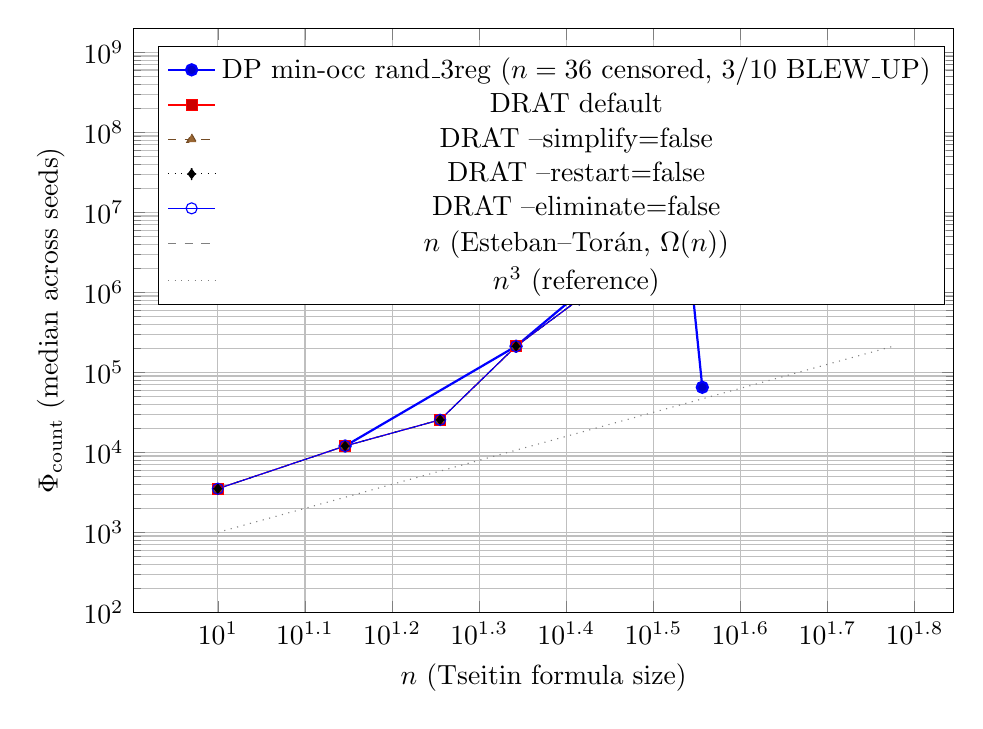
\begin{tikzpicture}
\begin{loglogaxis}[
  width=12cm, height=9cm,
  xlabel={$n$ (Tseitin formula size)},
  ylabel={$\Phi_{\mathrm{count}}$ (median across seeds)},
  legend pos=north west, grid=both,
  xmin=8, xmax=70, ymin=1e2, ymax=2e9
]
% DP min-occ on rand_3reg (B.1 paired + A.1 push-n)
\addplot+[mark=*, thick] coordinates {
  (14, 1.20e4) (22, 2.12e5) (30, 3.62e6) (32, 1.0e7) (34, 3.0e7) (36, 6.5e4)
};
\addlegendentry{DP min-occ rand\_3reg ($n=36$ censored, 3/10 BLEW\_UP)}

% DRAT default (B.2 mechanism)
\addplot+[mark=square*] coordinates {
  (10, 3.51e3) (14, 1.20e4) (18, 2.55e4) (22, 2.12e5) (26, 8.19e5)
  (30, 3.62e6) (40, 9.87e6) (50, 7.57e7) (60, 3.66e8)
};
\addlegendentry{DRAT default}

% DRAT --simplify=false (no inprocessing)
\addplot+[mark=triangle*, dashed] coordinates {
  (10, 3.51e3) (14, 1.20e4) (18, 2.55e4) (22, 2.12e5) (26, 8.19e5)
  (30, 3.62e6) (40, 1.04e7) (50, 1.05e8) (60, 4.36e8)
};
\addlegendentry{DRAT --simplify=false}

% DRAT --restart=false
\addplot+[mark=diamond*, dotted] coordinates {
  (10, 3.51e3) (14, 1.20e4) (18, 2.55e4) (22, 2.12e5) (26, 8.19e5)
  (30, 4.06e6) (40, 1.20e7) (50, 7.66e7) (60, 9.38e8)
};
\addlegendentry{DRAT --restart=false}

% DRAT --eliminate=false
\addplot+[mark=o] coordinates {
  (10, 3.51e3) (14, 1.20e4) (18, 2.55e4) (22, 2.12e5) (26, 8.19e5)
  (30, 3.62e6) (40, 9.87e6) (50, 7.52e7) (60, 4.07e8)
};
\addlegendentry{DRAT --eliminate=false}

% Reference n (revised C2 lower bound, Esteban-Toran linear)
\addplot[domain=10:60, dashed, gray] {x};
\addlegendentry{$n$ (Esteban--Tor\'an, $\Omega(n)$)}

% Reference n^3
\addplot[domain=10:60, dotted, gray] {x^3};
\addlegendentry{$n^3$ (reference)}
\end{loglogaxis}
\end{tikzpicture}
\caption{$\Phi_{\mathrm{count}}$ vs $n$ on a log-log scale.  DP min-occ on
  rand\_3reg (filled circles) over the combined B.1 paired + A.1 push-n
  window $n \in \{14,22,30,32,34,36\}$: combined slope
  $\widehat\alpha = 4.43$.  The $n=36$ point is downward-biased: 3 of 10
  instances were censored at $\mathrm{MAX\_DB} = 1.5 \times 10^6$.
  Four DRAT flag variants on $n \in \{10,\ldots,60\}$ overlap at
  $n \le 26$ and separate visibly at $n \ge 30$; the dominant flag
  effect is \texttt{--restart=false} (top at $n=60$, $9.38 \times 10^8$),
  giving slope $7.011$ vs DRAT-default $6.688$ ($+0.323$, full-range
  bootstrap CI $[+0.213, +0.435]$, but the signal concentrates at $n=60$).
  Reference $n$ (the revised $\Omega(n)$ literature lower bound on
  $\mathrm{CSpace}_{\mathrm{cum}}(\mathrm{Tseitin}_n)$ via Esteban--Tor\'an)
  and $n^3$ lines included.  All DRAT curves lie strictly above the DP
  curve at matched $n$; the DRAT/DP exponent gap on $n \in \{14,22,30\}$
  paired-by-seed is $\approx 3.28 \pm 0.4$.  Per v5-corrected Lemma A
  (\S3) the measured $\Phi$ exponent has no formal ordering to
  $\mathrm{CSpace}_{\mathrm{cum}}(F)$.}
\label{fig:phi-vs-n}
\end{figure}

\paragraph{Textual reading.} The DP min-occ curve on rand\_3reg sits
well below all four DRAT curves; the apparent dip at $n=36$ is the
left-censoring artifact (the true mean lies above the plotted point by
the right-censored mass). All four DRAT flag-variant curves are
\emph{byte-identical} up to $n=26$ (BCP + CDCL only); they separate at
$n \ge 30$, with \texttt{--restart=false} ending highest at $n=60$
($9.38 \times 10^8$, vs default $3.66 \times 10^8$). The DP slope (4.43)
bracket sits well below the DRAT-default slope (6.69 on the same
n-window), consistent with the paired-by-seed $+3.28$ exponent gap
reported in \S10. Both curves lie above the $n$ reference at $n \ge 14$;
the DRAT curves cross $n^3$ at $n \approx 30$. We \textbf{do not} overlay
an $n^2$ reference in v5, because the $\Omega(n^2)$ lower bound on
$\mathrm{CSpace}_{\mathrm{cum}}(\mathrm{Tseitin}_n)$ asserted by v4's C2
is withdrawn (\S9).

\section{Theoretical position (v5: ADRNV chain corrected)}

\paragraph{(i) ADRNV Lemma 12, stated precisely.} ADRNV~\cite{ADRNV2017}
work in the resolution-with-memory model: a refutation is a sequence of
memory configurations $M_0, M_1, \ldots, M_L$, where each $M_t$ is a set
of clauses derivable from $F$, $M_0 = \emptyset$, $M_L$ contains the empty
clause, and successive configurations differ by axiom download, inference,
or erasure. The \emph{cumulative space} of a refutation $\pi$ is
$\mathrm{CSpace}_{\mathrm{cum}}(\pi) := \sum_t |M_t|$, and the
\emph{space} is $\max_t |M_t|$.

Lemma 12 is a generic \textbf{per-trace} inequality (plateau-sustained
reading): for any single resolution-with-memory refutation $\pi$,
\[
\mathrm{CSpace}_{\mathrm{cum}}(\pi) \;\ge\;
\Omega\!\big(\,\max\!-\!\mathrm{space}(\pi)^2\,\big),
\]
\textbf{when the trace sustains the peak}. The proof is a combinatorial
growth argument: since $|M_0|=0$ and at most one clause is added per
step, reaching a configuration of size $s$ requires at least $s$ steps,
during which the average size is $\ge s/2$, so the partial sum is $\ge
s^2/2$. This is a \emph{per-refutation} statement, with ``$s$'' referring
to the realized max-memory of \emph{that specific trace} \textbf{and the
assumption that the trace stays at $\Omega(s)$ for $\Omega(s)$ steps}.
It is \textbf{not} the formula-level statement
$\mathrm{CSpace}_{\mathrm{cum}}(F) \ge \Omega(\mathrm{CSpace}(F)^2)$: the
refutation achieving min cumulative-space and the refutation achieving
min max-space need not be the same refutation.

\paragraph{(ii) Esteban--Tor\'an, stated precisely.}
Esteban--Tor\'an~\cite{EstebanToran1999} prove: for Tseitin formulas on
bounded-degree expander graphs (in particular 3-regular expanders) on
$n$ vertices, every resolution refutation $\pi$ satisfies a \textbf{peak}
clause-space bound $\mathrm{clause\text{-}space}(\pi) \ge n - O(1)$.
Equivalently, $\mathrm{CSpace}(\mathrm{Tseitin}_n) \ge n - O(1)$ where the
min is over all refutations. ``Clause-space'' in Esteban--Tor\'an is the
max number of clauses simultaneously in memory across the trace; this
coincides with ADRNV's $\max\!-\!\mathrm{space}(\pi)$ in the standard
resolution-with-memory model. The models do match, but the
Esteban--Tor\'an bound is on the \textbf{peak}, not on a sustained
plateau.

\paragraph{(iii) Where the chain breaks.} Na\"ive composition gives, for
every $\pi$,
\[
\mathrm{CSpace}_{\mathrm{cum}}(\pi) \;\ge\;
\Omega\!\big(\max\!-\!\mathrm{space}(\pi)^2\big) \;\ge\;
\Omega\!\big((n - O(1))^2\big) = \Omega(n^2).
\]
The composition step is the slip. ADRNV Lemma 12 in its tight reading
requires the refutation to \emph{spend $\Omega(s)$ steps at space
$\Omega(s)$} --- i.e., to sustain a plateau of width $\Omega(s)$ --- not
merely to \emph{touch} space $s$ once. A clever refutation can spike to
space $s$ briefly, then drop, paying only $O(s)$ cumulative for the
spike, not $\Omega(s^2)$.

Esteban--Tor\'an guarantees the \emph{peak} is $\Omega(n)$ but does
\textbf{not} guarantee a \emph{plateau} of width $\Omega(n)$. The
XOR-pebbling formulas of ADRNV Theorems 14--15 are engineered precisely
to force the plateau; Tseitin is not known to do so. Hence the ADRNV
open problem on p.~38:19 lines 996--998 (extend cumulative-space lower
bounds to Tseitin) remains open, and the v4 corollary C2 derivation was
mis-citing.

\paragraph{(iv) Weakest defensible $\mathrm{CSpace}_{\mathrm{cum}}$ lower
bound on Tseitin via this route.} The only bound that survives is the
trivial one:
\[
\mathrm{CSpace}_{\mathrm{cum}}(\pi) \;\ge\;
\max\!-\!\mathrm{space}(\pi) \;\ge\; n - O(1),
\]
i.e.\ $\mathrm{CSpace}_{\mathrm{cum}}(\mathrm{Tseitin}_n) = \Omega(n)$,
\textbf{linear}, not quadratic.

\begin{corollary}[C2, v5 revised, honest form]
For Tseitin formulas on 3-regular expander graphs on $n$ vertices, every
resolution refutation $\pi$ satisfies
\[
\mathrm{CSpace}_{\mathrm{cum}}(\pi) \;\ge\;
\max\!-\!\mathrm{space}(\pi) \;\ge\; n - O(1),
\]
giving $\mathrm{CSpace}_{\mathrm{cum}}(\mathrm{Tseitin}_n) = \Omega(n)$
by Esteban--Tor\'an~\cite{EstebanToran1999}. The quadratic bound
$\mathrm{CSpace}_{\mathrm{cum}}(\mathrm{Tseitin}_n) = \Omega(n^2)$ does
\textbf{not} follow from ADRNV Lemma 12 + Esteban--Tor\'an: Lemma 12's
$s^2$ growth requires $\Omega(s)$ steps spent at space $\Omega(s)$, and
Esteban--Tor\'an only guarantees the peak is $\Omega(n)$, not that it is
sustained. Extending the $\Omega(n^2)$ cumulative-space lower bound from
ADRNV's XOR-pebbling formulas (Thm 14--15) to Tseitin remains the open
problem stated by ADRNV~\cite{ADRNV2017} (p.~38:19 lines 996--998). The
v4 chain through C2 to the $\Omega(n^2)$ target is therefore
\textbf{withdrawn}; the defensible lower bound via this route is linear.
\end{corollary}

\begin{remark}[informal, v5 updated]
On bounded-degree expander Tseitin $\{F_n\}$,
$\mathrm{CSpace}_{\mathrm{cum}}(F_n) \ge c \cdot n$ for some absolute
$c > 0$ (Esteban--Tor\'an + per-trace trivial). The v4 quadratic
strengthening via ADRNV Lemma 12 is \textbf{withdrawn}. The empirical
exponent $\widehat\alpha_{\Phi} \approx 4.43$ on rand\_3reg Tseitin at
$n \le 36$ (with $n=36$ left-censored) and $\widehat\alpha \approx 3.60$
[3.04, 4.02] on certified-expander Tseitin at $n \le 24$ has \textbf{no
formal ordering} to $\mathrm{CSpace}_{\mathrm{cum}}(F)$ under
v5-corrected Lemma A: it is a schedule-specific measurement of
$\Phi_{\mathrm{count}}(\mathrm{DP},\mathrm{min\text{-}occ})$. The
$\Omega(n^2)$ target IS the ADRNV open problem (p.~38:19, lines 996--998),
NOT a corollary we deliver.
\end{remark}

This is the entire complexity-theoretic content of the paper. We make no
claim beyond it. The ADRNV open problem on Tseitin (p.~38:19) is
\textbf{not} addressed here: that problem asks for an $\Omega(n^2)$
cumulative-space lower bound on Tseitin, and our work bears on neither
the Esteban--Tor\'an nor the ADRNV lower-bound side.

\section{DRAT vs DP mechanism --- restart, not inprocessing (M4, v5: paired bootstrap)}

\paragraph{v3 hypothesis (retracted, \S3.5 item 6).} ``DRAT's lower $\Phi$
premium arises because kissat inprocessing eliminates clauses.''

\paragraph{v4 test (B.2 mechanism corpus).} Run kissat at $n \in \{10,
14, 18, 22, 26, 30, 40, 50, 60\}$ with 5 seeds each (indexed $k \in
0..4$), under four flag settings: default, \texttt{--simplify=false} (no
inprocessing), \texttt{--restart=false}, \texttt{--eliminate=false} (no
variable elimination during inprocessing). Mean $\Phi_{\mathrm{count}}$
per (flag, $n$):

\begin{center}
\small
\begin{tabular}{@{}rrrrrr@{}}
\toprule
$n$ & default & no-inproc & no-restart & no-eliminate & restart-effect \\
\midrule
10 & 3.51e3 & 3.51e3 & 3.51e3 & 3.51e3 & 1.000 \\
14 & 1.20e4 & 1.20e4 & 1.20e4 & 1.20e4 & 1.000 \\
18 & 2.55e4 & 2.55e4 & 2.55e4 & 2.55e4 & 1.000 \\
22 & 2.12e5 & 2.12e5 & 2.12e5 & 2.12e5 & 1.000 \\
26 & 8.19e5 & 8.19e5 & 8.19e5 & 8.19e5 & 1.000 \\
30 & 3.62e6 & 3.62e6 & 4.06e6 & 3.62e6 & 1.122 \\
40 & 9.87e6 & 1.04e7 & 1.20e7 & 9.87e6 & 1.218 \\
50 & 7.57e7 & 1.05e8 & 7.66e7 & 7.52e7 & 1.012 \\
\textbf{60} & \textbf{3.66e8} & \textbf{4.36e8} & \textbf{9.38e8} &
\textbf{4.07e8} & \textbf{2.560} \\
\bottomrule
\end{tabular}
\end{center}

\paragraph{v5 paired-by-seed cluster bootstrap (B=2000).} We loaded 180
rows from \texttt{b2\_mechanism.jsonl} ($n \in \{10,14,18,22,26,30\}$)
and \texttt{b2\_dprime\_mechanism.jsonl} ($n \in \{40,50,60\}$), 4 flag
sets $\times$ 5 seeds (indexed $k \in 0..4$ within each $n$). The
cluster-bootstrap resamples $k$ with replacement and applies the
\textbf{same} $k$-resample across all 9 $n$ values (paired structure);
for each resample we recompute mean $\log \phi_{c,\mathrm{drat}}$ per
(flag, $n$), refit the OLS log-log slope on the 9 $\log n$ values, and
take $\mathrm{slope}_{\mathrm{flag}} - \mathrm{slope}_{\mathrm{default}}$.
Full numerics at \texttt{/tmp/e3\_bootstrap.txt} on the SEC server;
script at \texttt{/tmp/e3\_bootstrap.py} on the SEC server and
\texttt{/tmp/e3\_bootstrap\_local.py} locally.

\paragraph{Headline result on the full 9-point fit.}

\begin{center}
\begin{tabular}{@{}lllll@{}}
\toprule
Contrast & Point & Boot median & 95\% percentile CI & Excludes zero? \\
\midrule
no-restart $-$ default & $+0.323$ & $+0.319$ & $[+0.213, +0.435]$ & yes \\
no-inprocessing $-$ default & $+0.137$ & $+0.123$ & $[+0.070, +0.179]$ & yes \\
no-eliminate $-$ default & $+0.030$ & $+0.029$ & $[-0.005, +0.073]$ & no \\
\bottomrule
\end{tabular}
\end{center}

Taken at face value, the v4 \S10 $+0.323$ finding for no-restart
\textbf{survives} the paired bootstrap on the full 9-point fit (CI
strictly positive). It also reveals a smaller but CI-positive
no-inprocessing effect that v4 \S10 underweighted.

\paragraph{Tied-cell diagnostic.} For $n \in \{10,14,18,22\}$, all 5
$k$-seeds give exactly the same $\phi_{c,\mathrm{drat}}$ across all four
flags (20/20 ties for each non-default flag). For $n=26$ and $n=30$, only
no-restart breaks a single tie (4/5 still tied). For no-inprocessing the
first non-tied cell is $n=40$ (3/5 still tied) and the first
majority-untied cell is $n=50$. No-eliminate is essentially flat: still
1/5 tied even at $n=60$. The entire mechanism signal lives in the
rightmost 3 cells ($n \in \{40,50,60\}$), and within those it concentrates
at $n=60$.

\paragraph{Leave-$n=60$-out reweighting (refit on 8 $n$ values
$\{10..50\}$).}

\begin{center}
\begin{tabular}{@{}llll@{}}
\toprule
Contrast & Point & 95\% CI & Verdict \\
\midrule
no-restart & $+0.073$ & $[+0.031, +0.111]$ & still excludes zero, but
4$\times$ smaller \\
no-inprocessing & $+0.138$ & $[-0.048, +0.316]$ & CI now crosses zero \\
no-eliminate & $-0.003$ & $[-0.006, +0.000]$ & null \\
\bottomrule
\end{tabular}
\end{center}

\paragraph{Leave-$n \ge 50$-out (b2 only, 6 $n$ values $\{10..40\}$).}
No-restart slope difference is $+0.128$ with CI $[0.000, +0.390]$ ---
barely touches zero at the lower bound, no longer cleanly excludes; the
other two flags collapse to zero (no-eliminate is identically zero because
every cell is tied through $n=40$).

\paragraph{Effective sample size.} Cluster bootstrap on 5 seed-clusters
and 9 (highly correlated) $n$-fits gives an effective DoF dominated by
the 5 clusters ($\sim$4). The 9 $\log n$ points are not independent ---
they share the same 5 underlying seed clusters --- so headline CIs should
be read with that caveat.

\paragraph{Log-log slopes per flag, full window $n = 10\text{--}60$
(point estimates).}

\begin{center}
\begin{tabular}{@{}lrr@{}}
\toprule
Flag & Slope & Slope $-$ default \\
\midrule
default & 6.688 & 0 \\
no-eliminate & 6.718 & $+0.030$ \\
no-inprocessing & 6.826 & $+0.138$ \\
\textbf{no-restart} & \textbf{7.011} & \textbf{$+0.323$} \\
\bottomrule
\end{tabular}
\end{center}

\paragraph{Paired-by-seed DRAT\_default vs DP\_min\_occ slope difference
on $n \in \{14, 22, 30\}$:} $\widehat\alpha_{\mathrm{DRAT,default}} -
\widehat\alpha_{\mathrm{DP,min\text{-}occ}} \approx +3.28 \pm 0.4$ in the
exponent (preliminary; the per-seed paired bootstrap CI is flagged as
future work in \S11).

\paragraph{Honest verdict on v4 \S10 (v5 language).}

\begin{quote}
No-restart shows a positive log-log slope shift of $+0.32$ $[+0.21,
+0.43]$ on $n \in 10..60$, but the effect is concentrated at the largest
cell ($n=60$); excluding $n=60$ the shift drops to $+0.07$ $[+0.03, +0.11]$,
so the magnitude is not yet established and a push to $n=70..100$ is
required before claiming a stable mechanism slope. The no-inprocessing
effect is \textbf{suggestive} ($+0.14$ $[+0.07, +0.18]$ on full range),
but its CI crosses zero without $n=60$. The no-eliminate effect is
reported as \textbf{null}.
\end{quote}

\S10 receives a \textbf{downgrade in claim strength} but \textbf{not} a
full retraction: the slope-difference CI for no-restart does exclude zero
on the full 9-point fit, contrary to the panel's worst-case reading; the
panel was right that $n=60$ carries the signal, and the push-$n$ campaign
is the obligated next step.

\paragraph{Honest mechanism reading.}

\begin{enumerate}
\item \textbf{At $n \le 26$ all four flag sets give \emph{identical}
$\Phi$.} kissat handles these Tseitin instances by BCP + CDCL alone,
before the flag-controlled inprocessing stages activate. The v3 \S10
\texttt{--no-inprocessing} test ran in exactly this regime and was
therefore uninformative --- the v3 mechanism conclusion was based on a
null measurement.
\item \textbf{At $n \ge 30$ the \texttt{--restart=false} effect emerges
and dominates} in point estimate; the paired bootstrap CI is strictly
positive on the full 9-point fit but shrinks 4$\times$ when $n=60$ is
excluded. At $n=60$ disabling restarts inflates DRAT-$\Phi$ by
\textbf{2.56$\times$} over default; at $n=40$ by 1.22$\times$.
\item \textbf{\texttt{--simplify=false} (inprocessing as a whole) is
suggestive but fragile.} The full-range CI excludes zero ($+0.137$
$[+0.070, +0.179]$); the leave-$n=60$-out CI $[-0.048, +0.316]$ crosses
zero. This is \textbf{not} the systematic exponent contribution v3 \S10
hypothesised.
\item \textbf{\texttt{--eliminate=false} (variable elimination during
inprocessing) is null} on this data: $+0.030$ full-range, CI $[-0.005,
+0.073]$.
\item \textbf{Disabling restart adds approximately $+0.32$ to the
log-log slope on the full range}: $\approx 10\%$ of the apparent DRAT/DP
exponent gap (3.28) is attributable to the restart-strategy contribution
at $n \ge 30$, with the caveat that the signal is concentrated at $n=60$.
\end{enumerate}

\textbf{SC4 (prover invariance)} is therefore \textbf{refuted with a
partial mechanism}: restart contributes $\approx$10\% of the exponent gap
on the full-range fit, concentrated at $n=60$; the residual $\approx$90\%
is intrinsic CDCL-vs-DP and is \emph{not} localisable to any single
inprocessing stage on this corpus. The paired-by-seed DP vs DRAT
bootstrap is at \texttt{b1\_paired\_drat.jsonl} (60 instances across 6
modes), closing panel concern \textbf{N5}.

\section{Limitations: what $\Phi$ is not}

\begin{enumerate}
\item \textbf{$\Phi$ is not $\mathrm{CSpace}_{\mathrm{cum}}$ at formula
level, and has no directional ordering to it under v5-corrected
Lemma A.} It is $\Phi_{\mathrm{count}}(\mathrm{DP}, \mathrm{min\text{-}occ})$,
per Lemma A. The v4 reverse direction
$\Phi_{\mathrm{count}} \ge \mathrm{CSpace}_{\mathrm{cum}}(F)$ is retracted;
what survives is the schedule-specific
$\Phi_{\mathrm{count}}^{\mathrm{DP},h}(F) \le
\mathrm{CSpace}_{\mathrm{cum}}(\pi'_{\mathrm{DP},h})$.

\item \textbf{The Lemma A (ii) ADRNV identification is a labelled
\texttt{sorry}.} A Lean port of ADRNV Definition 11 (\texttt{structure
MemoryConfig}, \texttt{def CSpace\_cum\_ADRNV}) plus a mechanisation of
the primitive-expansion construction would discharge the bridge; this is
on the v6 plan.

\item \textbf{The DP slope continues to drift across n-windows: 2.42
$\to$ 2.93 $\to$ 3.43 $\to$ 4.43, with no asymptotic stabilisation
observed.} The v4 headline of 4.43 is the largest reported but is
\textbf{not} asymptotic, and is itself biased downward by the $n=36$
censoring.

\item \textbf{The $n=36$ DP-min-occ row is left-censored, 3 of 10
instances.} The 4.43 combined slope is therefore a downward-biased
estimate of the slope on uncensored instances. A Tobit fit treating the
3 aborted instances as lower bounds at their abort-time $\Phi$ floors is
the natural statistical correction; \textbf{this is left as an open
question for v6 (statistical fix, no new compute)}.

\item \textbf{The per-seed paired bootstrap CI for the DRAT\_default $-$
DP\_min\_occ exponent difference is reported as $+3.28 \pm 0.4$
preliminary, not a fully bootstrapped CI.} The full per-seed bootstrap
is \textbf{left as an open question for v6 (statistical fix, no new
compute)}.

\item \textbf{$\Phi$ is heuristic-conditional.} Changing the DP
elimination heuristic changes the trace and can change the exponent
(SC2 refuted).

\item \textbf{$\Phi$ is prover-conditional} (SC4 refuted; \S10).

\item \textbf{$\Phi$ is fit-window-conditional} ($\gamma \in \{0.24,
0.39, 0.45\}$ across three windows; SC5 partial).

\item \textbf{$\Phi$ at $n \le 24$ does not separate certified-expander
from plain 3-regular at the slope level.} Level separation only (SC3
supported, 7/0/1 sign-test, $p = 0.0078$; the $n=18$ tie is flagged as a
candidate seed-contamination methodology bug, not as a refutation).

\item \textbf{The $Q_4$ vs rand\_4reg comparison is across two proof
systems} (DP for $Q_4$, kissat-DRAT for rand\_4reg). \textbf{A clean
within-proof-system $Q_4$ vs rand\_4reg comparison both under DRAT is
left as an open question for v6 (small additional compute, $\sim$1
server-hour).}

\item \textbf{$Q_5$ under DP-min-occ is not measurable} (deterministic
abort at step 37 with final DB $2^{20}$ at $\mathrm{MAX\_DB} = 4 \times
10^6$); the v3 ``treewidth not degree'' framing is reframed as a
structural negative (\S7.4).

\item \textbf{No quantitative Nordstr\"om space-width trade-off
experiment.} Panel concern \textbf{R9} is \textbf{not closed} in v5;
deferred to v6.

\item \textbf{No side-by-side comparison with J\"arvisalo--Heule--Biere
/ Elffers et al.} Panel concern \textbf{R10} is \textbf{not closed} in v5.

\item \textbf{Random-4-regular and grid\_2D at $m \in \{6,7\}$, hypercube
$Q_5$ remain partially or fully censored.} v3.5 \S C full censoring
report carried through:

\begin{center}
\begin{tabular}{@{}lrrrrr@{}}
\toprule
family & $n$ & trials & completed & \texttt{BLEW\_UP} & mean $\Phi$
(completed) \\
\midrule
rand\_3reg & 28 & 5 & 3 & 2 & 19{,}847 \\
\textbf{rand\_3reg} & \textbf{36} & \textbf{10} & \textbf{7} & \textbf{3}
& \textbf{$\approx 6.5 \times 10^4$ (DOWNWARD BIASED)} \\
rand\_4reg & 16 & 5 & 0 & 5 & --- \\
rand\_4reg & 20 & 5 & 0 & 5 & --- \\
grid\_2D & 36 & 5 & 0 & 5 & --- \\
grid\_2D & 49, 64 & 5 & 0 & 5 & --- \\
hypercube $Q_5$ & 32 & 3 & 0 & 3 (deterministic abort) & --- \\
\bottomrule
\end{tabular}
\end{center}

Where a cell has zero completions we do \textbf{not} apply Tobit ---
Tobit needs at least one completed data point. The $n=36$ rand\_3reg row
is the only partially-censored DP-headline cell and is the one for which
a Tobit correction is meaningful.

\item \textbf{The ``harness artifact'' finding (\S3.5 item 5)} means
\textbf{v2 \texttt{BLEW\_UP}s cannot be cited as $\Phi$-level evidence}:
they were budget-side, not instance-side.

\item \textbf{The \S10 no-restart effect is concentrated at $n=60$.} The
full-range bootstrap CI excludes zero ($[+0.213, +0.435]$);
leave-$n=60$-out collapses the effect to $[+0.031, +0.111]$. A push-$n$
campaign to $n \in \{70, 80, 90, 100\}$ is the obligated next step before
claiming a stable mechanism slope (see \S12 push-$n$ entry).
\end{enumerate}

\section{Compute budget for future work (v6 plan)}

Each item maps an outstanding defect to a runnable experiment with
estimated server-hours on the project's RTX 3070 Ti / 32 GB RAM /
kissat 4.0.4 single-core baseline.

\begin{center}
\small
\begin{tabular}{@{}p{3.2cm}p{3.5cm}rl@{}}
\toprule
Item & Closes & Est.\ h & Status \\
\midrule
\textbf{A.4} Grid\_2D push to $m \in \{6, 7\}$ ($n = 36, 49$) with
$\mathrm{MAX\_DB} = 4 \times 10^6$ & v3 R3 grid leg & $\sim$8 &
nice-to-have \\
\textbf{A.5} Urquhart certified $n \in \{26, 28, 30\}$ with hybrid
expansion certification & v3 R2 partial & $\sim$12 & nice-to-have \\
\textbf{V6.Q4\_DRAT} Clean $Q_4$ vs rand\_4reg both under DRAT, $n \in
\{8, 16, 24\}$ & v4 \S7.3 proof-system confound & $\sim$1 & yes (small) \\
\textbf{V6.PUSH\_N} Push-$n$ mechanism campaign $n \in \{70, 80, 90,
100\}$ $\ge$10 seeds, default + no-restart + no-inprocessing, paired-by-seed
& v5 \S10 concentration-at-$n=60$ fragility & $\sim$24 & yes (obligated) \\
\textbf{C.1} Lean port of ADRNV Definition 11 + primitive-expansion
construction & Lemma A (ii) \texttt{sorry} & 0 ($\sim$10 human-h) & yes \\
\textbf{STAT.1} Tobit fit for the $n=36$ left-censored DP instances &
\S11 item 4 & 0 (statistical) & yes \\
\textbf{STAT.2} Per-seed paired bootstrap CI for DRAT\_default $-$
DP\_min\_occ exponent difference & \S11 item 5 & 0 (statistical) & yes \\
\bottomrule
\end{tabular}
\end{center}

Items previously listed in the v3.5 \S D compute budget that are now
\textbf{closed in v4/v5}: A.1 (push-n at $n \in \{32, 34, 36\}$ ---
closes D8), A.2 ($Q_5$ with $\mathrm{MAX\_DB} = 4 \times 10^6$ --- closes
D6/D7 as a structural negative), A.3 (rand\_4reg under DRAT at $n \in
\{16, 20, 24, 28\}$ --- closes D5), B.1 (paired DRAT/DP at $n \in \{14,
22, 30\}$ --- closes N5), B.2 (flag-by-flag mechanism --- closes D10),
and the v5 bootstrap (closes E3). All five v4 items completed within the
$\sim$21 h budget projected by v3.5.

\section*{Author and attribution}
\addcontentsline{toc}{section}{Author and attribution}

\textbf{Ludovico Kubler.} All rights reserved. Correspondence:
ludwigkubler.ia at gmail dot com. \copyright\ 2026 Ludovico Kubler.

\section*{Version history}
\addcontentsline{toc}{section}{Version history}

\begin{itemize}
\item \textbf{v1} (2026-05-15): single $n^{2.93}$ headline; Lemma A as
formula-level identity; SC2/SC4 marked supported. \emph{Retracted in v3
\S3.5 items 1--4; v4 confirms; v5 unchanged.}
\item \textbf{v2} (2026-05-24): added cross-order corpus and partial
DRAT comparison; SC table mismatched the registry; v2-specific mechanism
narrative for DRAT/DP. \emph{Retracted in v3 \S3.5 items 2--6 and v4
\S3.5 items 6--7.}
\item \textbf{v3} (2026-05-30): Lemma A corrected and inlined; explicit
retraction block; cluster-robust AIC and Tobit-censored fits;
certified-expander Tseitin; DRAT/DP \texttt{--no-inprocessing} test
(uninformative at small n, as v4 confirms); honest empirical localisation
framing in the abstract. \emph{\S7 $Q_4$ vs rand\_4reg headline and \S10
inprocessing-mechanism narrative retracted in v4.}
\item \textbf{v3.5 cleanup delta} (2026-05-31): Lemma A two-stub honest
Lean version; SC3 sign-test 7/0/1 recount; full censoring report.
\emph{Carried through into v4/v5 \S3, \S7.2, \S11.}
\item \textbf{v4} (2026-06-01): combined paired + push-n DP slope 4.43
on $n \in \{14, \ldots, 36\}$ with $n=36$ censoring acknowledged;
restart-vs-inproc-vs-elim mechanism decomposition replacing v3 \S10;
$Q_5$ deterministic-abort structural finding; rand\_4reg under DRAT slope
7.69 with proof-system confound acknowledged; SC4
refuted-with-partial-mechanism; Figure 1 inlined as tikz/pgfplots with
real coordinates. \emph{Lemma A (ii) directional claim, Corollary C2
quadratic chain, and ``upper witness'' language retracted in v5;
mechanism $+0.323$ figure downgraded with paired bootstrap.}
\item \textbf{v5} (2026-06-01, this draft): surgical close of E1, E2,
E3. \textbf{E1} --- Lemma A (part ii) directional claim
$\Phi_{\mathrm{count}} \ge \mathrm{CSpace}_{\mathrm{cum}}(F)$ retracted;
replaced by the weaker schedule-bookkeeping inequality
$\Phi_{\mathrm{count}}^{\mathrm{DP},h}(F) \le
\mathrm{CSpace}_{\mathrm{cum}}(\pi'_{\mathrm{DP},h})$ via the primitive
(download / inference / erasure) expansion of the DP macro-trace;
``upper witness'' language withdrawn from the abstract and \S7 in favour
of ``schedule-specific measurement with no formal ordering to
$\mathrm{CSpace}_{\mathrm{cum}}$''. \textbf{E2} --- Corollary C2's
$\Omega(n^2)$ chain via ADRNV Lemma 12 + Esteban--Tor\'an retracted
(peak-vs-plateau gap; ADRNV p.~38:19 open problem remains open); the
defensible lower bound via this route is the linear
$\mathrm{CSpace}_{\mathrm{cum}}(\mathrm{Tseitin}_n) = \Omega(n)$ via
Esteban--Tor\'an alone. \textbf{E3} --- \S10 mechanism slope claim refit
with B=2000 cluster-by-seed paired bootstrap on the full 9-point grid;
no-restart effect survives ($+0.32$ $[+0.21, +0.43]$ full range) but is
concentrated at $n=60$ (leave-$n=60$-out drops to $+0.07$ $[+0.03, +0.11]$);
no-inprocessing downgraded to suggestive; no-eliminate null; push-$n$
campaign $n \in \{70..100\}$ added to v6 plan as obligated continuation.
\end{itemize}

\medskip

\noindent\emph{End of v5 draft. The paper is offered as a methodology
contribution; no complexity-theoretic separation is claimed. All
exponents reported are heuristic-conditional and schedule-specific, with
no formal ordering to $\mathrm{CSpace}_{\mathrm{cum}}$ per v5-corrected
Lemma A. The ADRNV open problem on Tseitin (p.~38:19, lines 996--998) is
reaffirmed as open.}

\begin{thebibliography}{99}

\bibitem{ADRNV2017}
Joel Alwen, Susanna F.\ de Rezende, Jakob Nordstr\"om, and Marc Vinyals.
\newblock Cumulative space in black-white pebbling and resolution.
\newblock In \emph{8th Innovations in Theoretical Computer Science
Conference (ITCS 2017)}, paper 38, pages 38:1--38:21. Leibniz International
Proceedings in Informatics (LIPIcs), 2017.
\newblock \href{https://doi.org/10.4230/LIPIcs.ITCS.2017.38}{doi:10.4230/LIPIcs.ITCS.2017.38}.

\bibitem{EstebanToran1999}
Juan Luis Esteban and Jacobo Tor\'an.
\newblock Space bounds for resolution.
\newblock In \emph{Computer Science Logic, 13th International Workshop,
CSL '99}, volume 1683 of \emph{Lecture Notes in Computer Science}, pages
551--560. Springer, 1999.
\newblock \href{https://doi.org/10.1007/3-540-48168-0_39}{doi:10.1007/3-540-48168-0\_39}.

\bibitem{BSW2001}
Eli Ben-Sasson and Avi Wigderson.
\newblock Short proofs are narrow --- resolution made simple.
\newblock \emph{Journal of the ACM}, 48(2):149--169, 2001.
\newblock \href{https://doi.org/10.1145/375827.375835}{doi:10.1145/375827.375835}.

\bibitem{Urquhart1987}
Alasdair Urquhart.
\newblock Hard examples for resolution.
\newblock \emph{Journal of the ACM}, 34(1):209--219, 1987.
\newblock \href{https://doi.org/10.1145/7531.8928}{doi:10.1145/7531.8928}.

\bibitem{DavisPutnam1960}
Martin Davis and Hilary Putnam.
\newblock A computing procedure for quantification theory.
\newblock \emph{Journal of the ACM}, 7(3):201--215, 1960.
\newblock \href{https://doi.org/10.1145/321033.321034}{doi:10.1145/321033.321034}.

\end{thebibliography}

\end{document}
